%=========================================
% 	   Einleitung     		 =
%=========================================

\chapter{SDH Versuch}
\section{Allgemeine Beschreibung der Versuche}
%Kurze Einleitung ins Thema
Der folgende Versuch handelt von der Multiplextechnik SDH. SDH steht Synchrone Digitale Hierarchie die es möglich macht niederratige Datenströme zu einem hochrratigen Datenstrom zu multiplexen, das Netz taktet dabei vollkommen synchron. In unserem Versuchsaufbau werden wir absichtlich verschiedene Fehler einspeisen sowie uns die Pointeraktivitäten im Netz genauer ansehen. Die Möglichkeit Fehler einzuspeisen wird uns durch das Messgerät GN Elmi EST 2100 ermöglicht, der ebenfalls als Multiplexer fungiert. Das Auswerten dieser Fehler ist über die Software Telecommunications-Management-Network-Software von Siemens gegeben. Der Rechner auf dem die Software läuft ist über die QST-E3 Schnittstelle mit den SMA 16 Multiplexern verbunden und sammelt so die nötigen Daten. 
Die Multiplexer unter sich sind mit Lichtwellenleiter verbunden die theoretisch eine Entfernung von gut 50Km schaffen würden. Da Elmi leider nicht von Siemens ist, ist es auch nicht möglich direkt über die Software zu sehen wie Elmi sich als Multiplexer verhält.

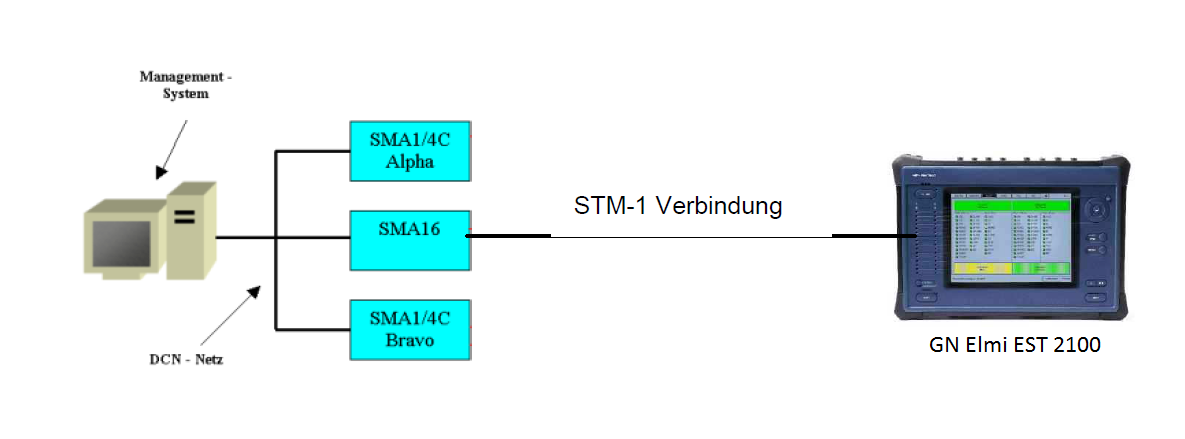
\includegraphics[scale=1]{sdh/versuchsaufbau.png} 

\section{Versuchsgegenstände im Detail}
Im folgenden betrachten wir uns die TMNS und Elmi für das Verständnis den den Umgang etwas genauer.

\subsection{GN Elmi EST 2100}
Elmi ist ein Messgerät das direkt mit den anderen Multiplexern über einen Lichtwellenleiter angeschlossen ist. Er fungiert in erster Linie zum einspeisen von Fehlern ins Netz um zu betrachten wie sich das SDH darauf verhält. Wie oben bereits erwähnt ist er selbst ebenfalls Teil des Netzes in Form von einem Multiplexers. Folgende Grafiken erläutern wie mit dem Gerät um zu gehen ist.
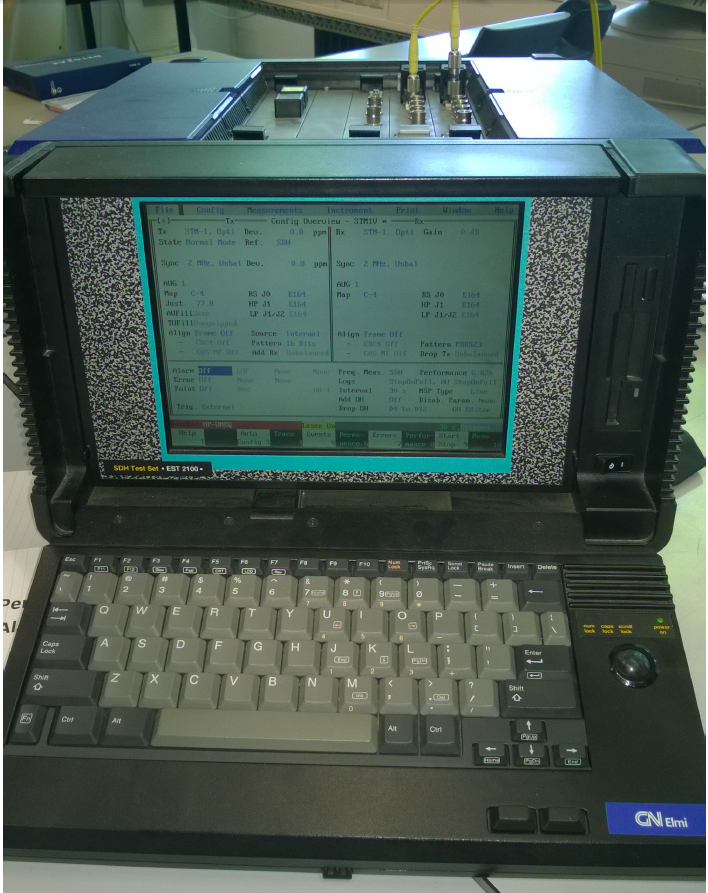
\includegraphics[scale=1]{sdh/elmi_start.png} 

Es gibt es veschiedene Möglichkeiten das Netz zu beeinflussen. Da Elmi einen eigenen internen Systemtakt besitzt, kann man diesen auch verwenden um so beispielsweise zwei verschiedene Takte im Netz zu simulieren. Unter den Menüpunkt Ref. kann man diesen dann beeinflussen.

\todo{Bild von Taktmenu}

Desweiteren für unseren Versuch wichtige Funktion bietet die Sektion ALARM. Hier kann man nach belieben Fehler ins Netz einspeisen. Diese kann man entweder als Burst, das bedeutete über einen bestimmten Zeitrahmen, oder kontinuierlich setzen. Für unserem Versuch werden nur diese zwei Sektionen benötigt deswegen wird hier nicht weiter auf die Funktionalität von Elmi eingegangen.
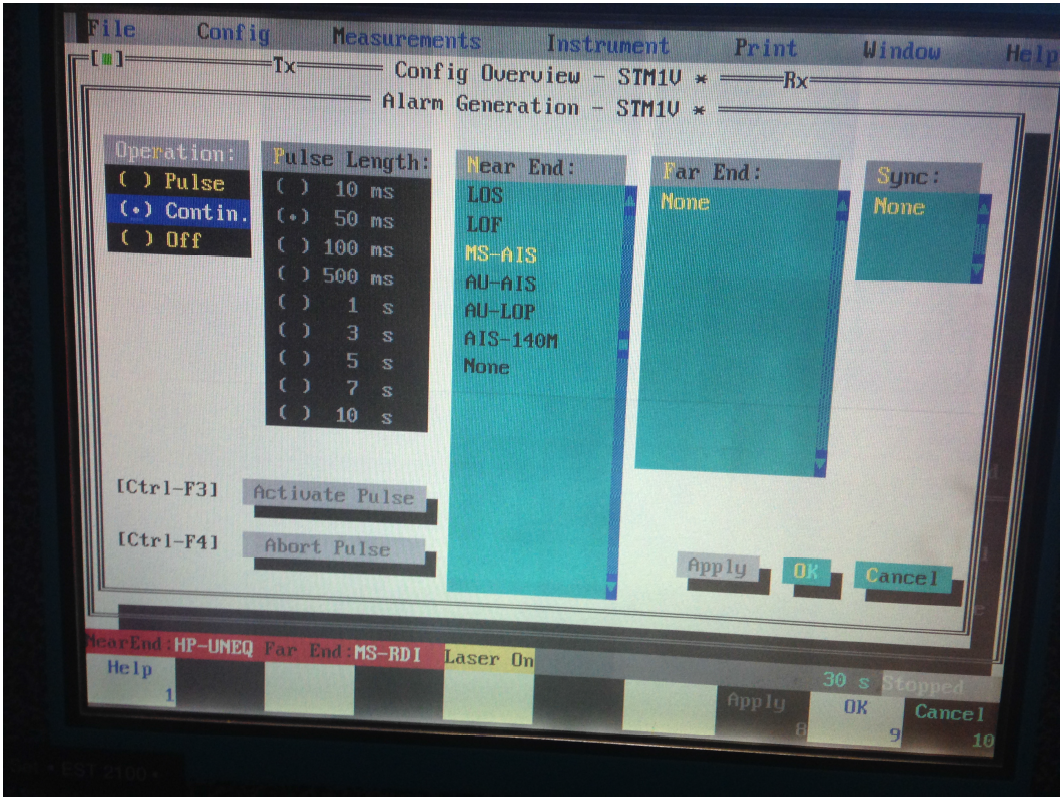
\includegraphics[scale=1]{sdh/elmi_fehler.png}  

\subsection{TMNS}
Die TMNS ist zur Analyse und Überwachung des SDH-Netzes hilfreich. In der Hauptansicht wird das Netz abstrakt für eine gute Übersicht dargestellt. Klickt man nun auf unser Testnetz \textit{Köln}
auf die Performancemessung gelangt man in die für den Versuch interessante Performanceansicht. \todo{stimmt das?}
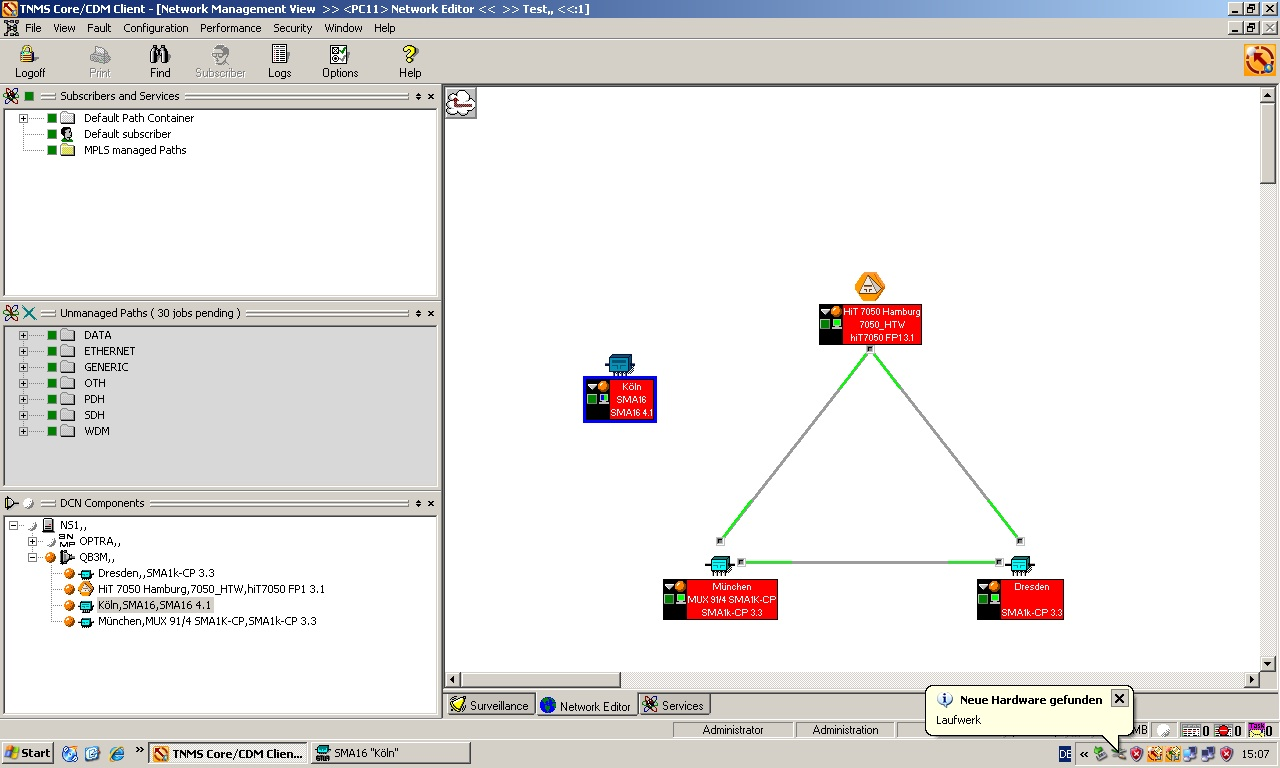
\includegraphics[scale=1]{sdh/tnms.bmp} 

Im Hauptfenster werden sämtliche Komponenten angezeigt die zu dem Netz gehören bis auf Elmi. Hier werden bei einkommenden Fehlern, durch rotes blinken markiert welche Komponente einen Fehler aufweist. In der Folgenden Abbildung ist zu sehen wie die Komponente in dem Steckplatz 406 auf Port 3 einen einkommenden Fehler anzeigt. Port 1 und 2 sind ebenfalls rot markiert jedoch weil die Ports konfiguriert sind aber kein Kabel angeschlossen ist. Also können wir diese einfach ignorieren. 
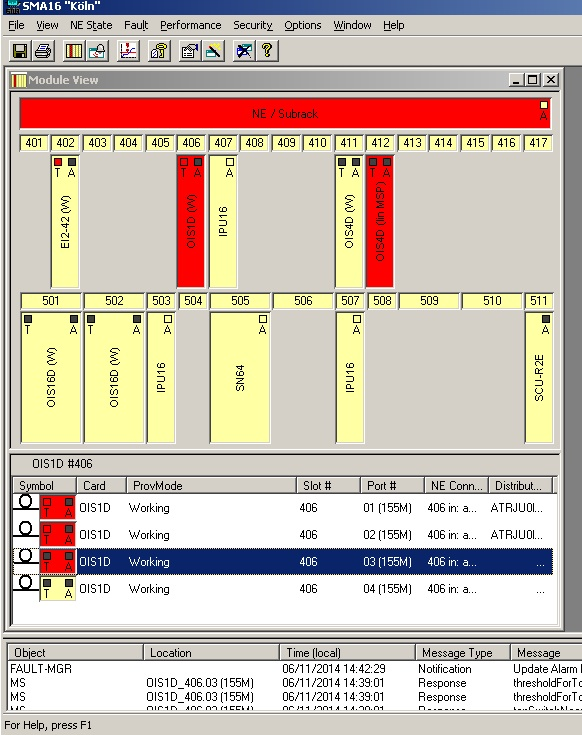
\includegraphics[scale=1]{sdh/Fehler2.bmp} 

Bei einem ankommenden Fehler kann man sich nun die Komponente genauer anschauen indem man den entsprechenden Port sich unter die Lupe nimmt. Durch Auswahl der Submenu-View gelangt man in eine Ansicht in der man genauer sehen kann wo der Fehler entstanden ist. 

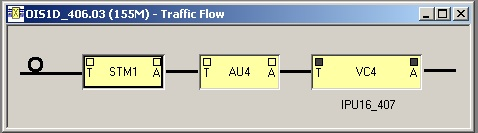
\includegraphics[scale=1]{sdh/komponent-performance.bmp} 

Hier hat man nun je nach Fehler die Auswahl. Wenn es um Pointer geht wird hier im Normalfall das AU-4 Fenster anfangen zu Blinken, wenn ein Netz-Fehler auftritt das STM-1 Fenster.
Diese schauen wir uns hier noch im Detail an.
Zuerst sehen wir hier die Performance-Ansicht von dem AU-4 Fenster.

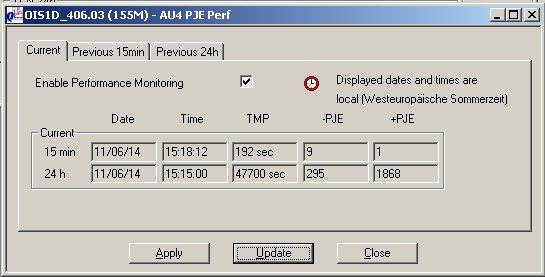
\includegraphics[scale=1]{sdh/Pointerview_detail.bmp} 
%zur pointerview was schreiben
Dieses beinhaltet:

\begin{itemize}
\item Date - Das Aktuelle Datum
\item Time - Die Aktuelle Zeit
\item TMP - Dauer des gemessenen Intervalls
\item -PJE - Die gezählten Negativ Pointer-Vorgänge
\item +PJE - Die gezählten Positiv Pointer-Vorgänge
\end{itemize}

Die Aktualisierung der Daten findet nur manuell mit dem Update Knopf statt. TMP ist hier im Auge zu behalten da die Daten alle 15 Minuten in eine Log-Datei geschrieben werden. Die Log-Dateien sind in den Reitern \textit{Previous 15min} und \textit{Previous 24h} wieder zu finden. 

Um im genau zu sehen was im STM-1 vor sich geht kann man sich hier ebenfalls die Performance-Ansicht anzeigen lassen. 
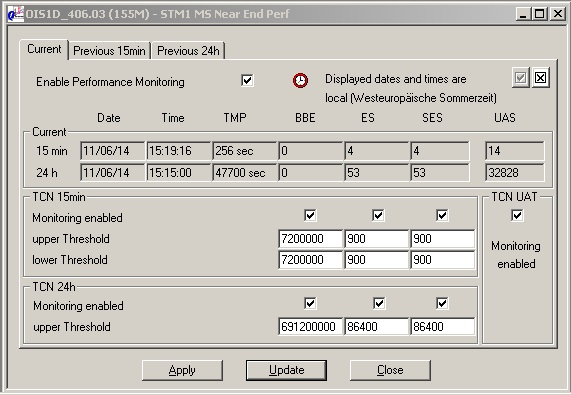
\includegraphics[scale=1]{sdh/ms-near-end.bmp} 

Folgende Daten werden angezeigt:

\begin{itemize}
\item Date - Das Aktuelle Datum
\item Time - Die Aktuelle Zeit
\item TMP - Dauer des gemessenen Intervalls
\item BBE - Background Block Error
\item ES - Errored Seconds
\item SES - Severely Errored Seconds
\item UAS - Unavailable Seconds
\end{itemize}

Was das Aktualisieren und das wegschreiben in die Log-Datei angeht ist der Vorgang wie bereits vorher beschrieben der Fall. 
Die Fehlerrate wird in Error-Sekunden angegeben die unterschiedliche Aussagen über den Fehler angeben.

\begin{itemize}
\item ES - beinhaltet,innerhalb einer Sekunde, ein oder mehrere fehlerhafte Blöcke. 
\item SES - beinhaltet, innerhalb einer Sekunde, 30 Prozent fehlerhafte Blöcke.
\item UAS - Nach 11 SES gilt eine Leitung als nicht mehr verfügbar. Im gegenzug gilt sie als vergügbar, nach 11 Sekunden ohne SES.
\end{itemize}




\section{Fehlereinspeisung}
Nachdem wir alle für den Versuch erforderlichen Komponenten kennengelernt haben, können wir nun den eigentlichen Versuch weiter beschreiben. Im folgenden sollen drei verschiedene Fehlermeldungen mit Hilfe von Elmi einmal kontinuierlich und einmal als Bursts eingespeist werden. Wenn im empfagenen Signal Bitfehler enthalten sind sendet der Empfänger eine Alarm-Nachricht in Senderichtung zurück. Bei dieser Rückmeldung spricht man von REI (Remote Error Indication). Die für uns wichtigen sind:

\begin{itemize}
\item LOS - Lost of Singnal, Rückgang der eingehenden optischen Leistungspegel, verursacht hohe Bitfehlerrate
\item MS-AIS - Multiplex Section Alarm Indication Signal, wird ausgelöst wenn K2 (bits 6, 7, 8) auf 111 gesetzt ist für mehr als 3 Frames.
\item LOF - Lost of Frame tritt auf wenn das Signal für mehr als 3 ms OOF (Out of Frame) ist.
\item OOF - Out of Frame tritt auf wenn die Bytes A1 und A2 länger als 624 \mu s  fehlerhaft sind
\end{itemize}

Sind im empfangenen Signal Bitfehler enthalten, meldet der Sensor
BIP Errors. Da das nicht gleichbedeutend mit dem Ausfall der Verbindung
ist, spricht man von einer Anomalie, die in Senderichtung zurückgemeldet
wird. Die Rückmeldung wird als REI (Remote Error Indication)
bezeichnet.



\subsubsection{Kontinuierliches Fehlereinspeisen}
Zuerst werden wir die Fehler kontinuierlich einspeisen. Nach dem feuern der Fehler fängt die entsprechende Komponente an zu Blinken und wir klicken uns bis in das STM-1_performance-Fenster durch.

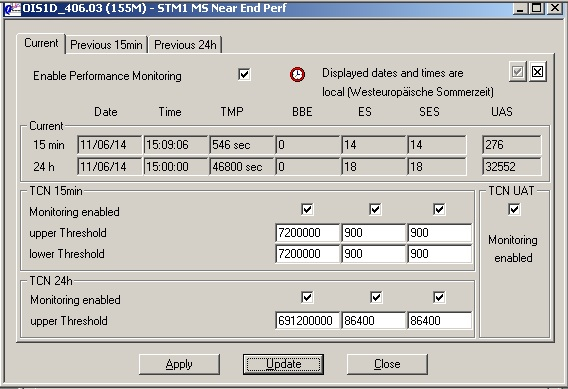
\includegraphics[scale=1]{sdh/stm1-konti.bmp} 

Die Ergebnisse sind alle wie zu erwarten gleich. Alle drei Fehlermeldungen lassen den UAS-Counter solange ansteigen bis man aufhört den Fehler einzuspeisen. Da alle drei Fehler kontinuierlich auftreten verursachen sie dauerhaft SES und somit nach kurzer Zeit UAS. Somit sind kontinuierliche Fehler sehr schwerwiegend und sofort zu behandeln.
Hier noch einmal ein Tabellarischer Überblick über alle gemessenen Daten:

\begin{tabular}
Fehlermeldung & Burst-Time & ES & SES & UAS & Fenster \\
MS-AIS & Kontinuierlich & 0 & 0 & ++ & STM1 \\
LOS & Kontinuierlich & 0 & 0 & ++ & STM1 \\
LOF & Kontinuierlich & 0 & 0 & ++ & STM1 \\
\end{tabular}

\subsubsection{Burst Fehlereinspeisung}

Als zweites Verursachen wir eine MS-AIS und ein LOS jeweils innerhalb von 100ms, einer Sekunde, und sieben Sekunden. 

\begin{tabular}
Fehlermeldung & Burst-Time & ES & SES & UAS & Fenster \\
MS-AIS & 100 ms & 1 & 1 & 0 &STM1 \\
MS-AIS & 1 s & 2 & 2 & 0 & STM1 \\
MS-AIS & 7 s & 8 & 8 & 0 & STM1 \\
LOS & 100 ms & 3 & 3 & 0 & STM1 \\
LOS & 1 s & 4 & 4 & 0 & STM1 \\
LOS & 7 s & 0 & 0 & 14 & STM1 \\
\end{tabular}

Wie man anhand der Tabelle sehen kann löst die MS-AIS lediglich maximal 8 SES aus und somit wird die Leitung nicht als Unavailable gesetzt.
Zu Beobachten war das bei den kruzen Bursts die TMNS überhaupt gar nicht auf den Fehler reagiert. Das ist erklärbar da bevor der Fehler erkannt wird, er bereits wieder vorbei ist. Bei den LOS Alarmen sind die Error Sekunden schon betrachtlich höher. Ein sieben Sekunden langer LOS kann die Leitung bereits für einige Momente ausser gefecht setzen wie man an dem UAS Feld erkennen kann. 

\subsection{Pointer}
Da das SDH-Netz ein voll getaktetes Netz ist und so durch Taktunterschiede es theoretisch zu einer Überlast kommen kann, gibt es Pointer. Dieser ist in der Administrative Unit zu finden und zeigt auf die Position der Nutzinfomrationen im Payload Bereich. Durch Pointer ist es möglich die Taktunterschiede, durch einfügen von Leer-Bytes oder früheres Senden von Payload, auszugleichen. Es können allerdings nur in jedem vierten Rahmen nach Ankündigung die Pointer angepasst werden.
In diesem Versuch beschäftigen wir uns mit dem dekrementieren und Inkrementieren von Pointern. Zusätlich dazu, werden wir mit dem Systemtakt des Netzes hantieren. 

\subsubsection{Manuelles negativ und positiv Justieren}
Elmi hat für die Justierung des Pointers ein eigenes Menu. Hier kann man einstellen ob man die Pointer-Justierung dauerhaft alle 1500 ms oder manuell durchführen will. 

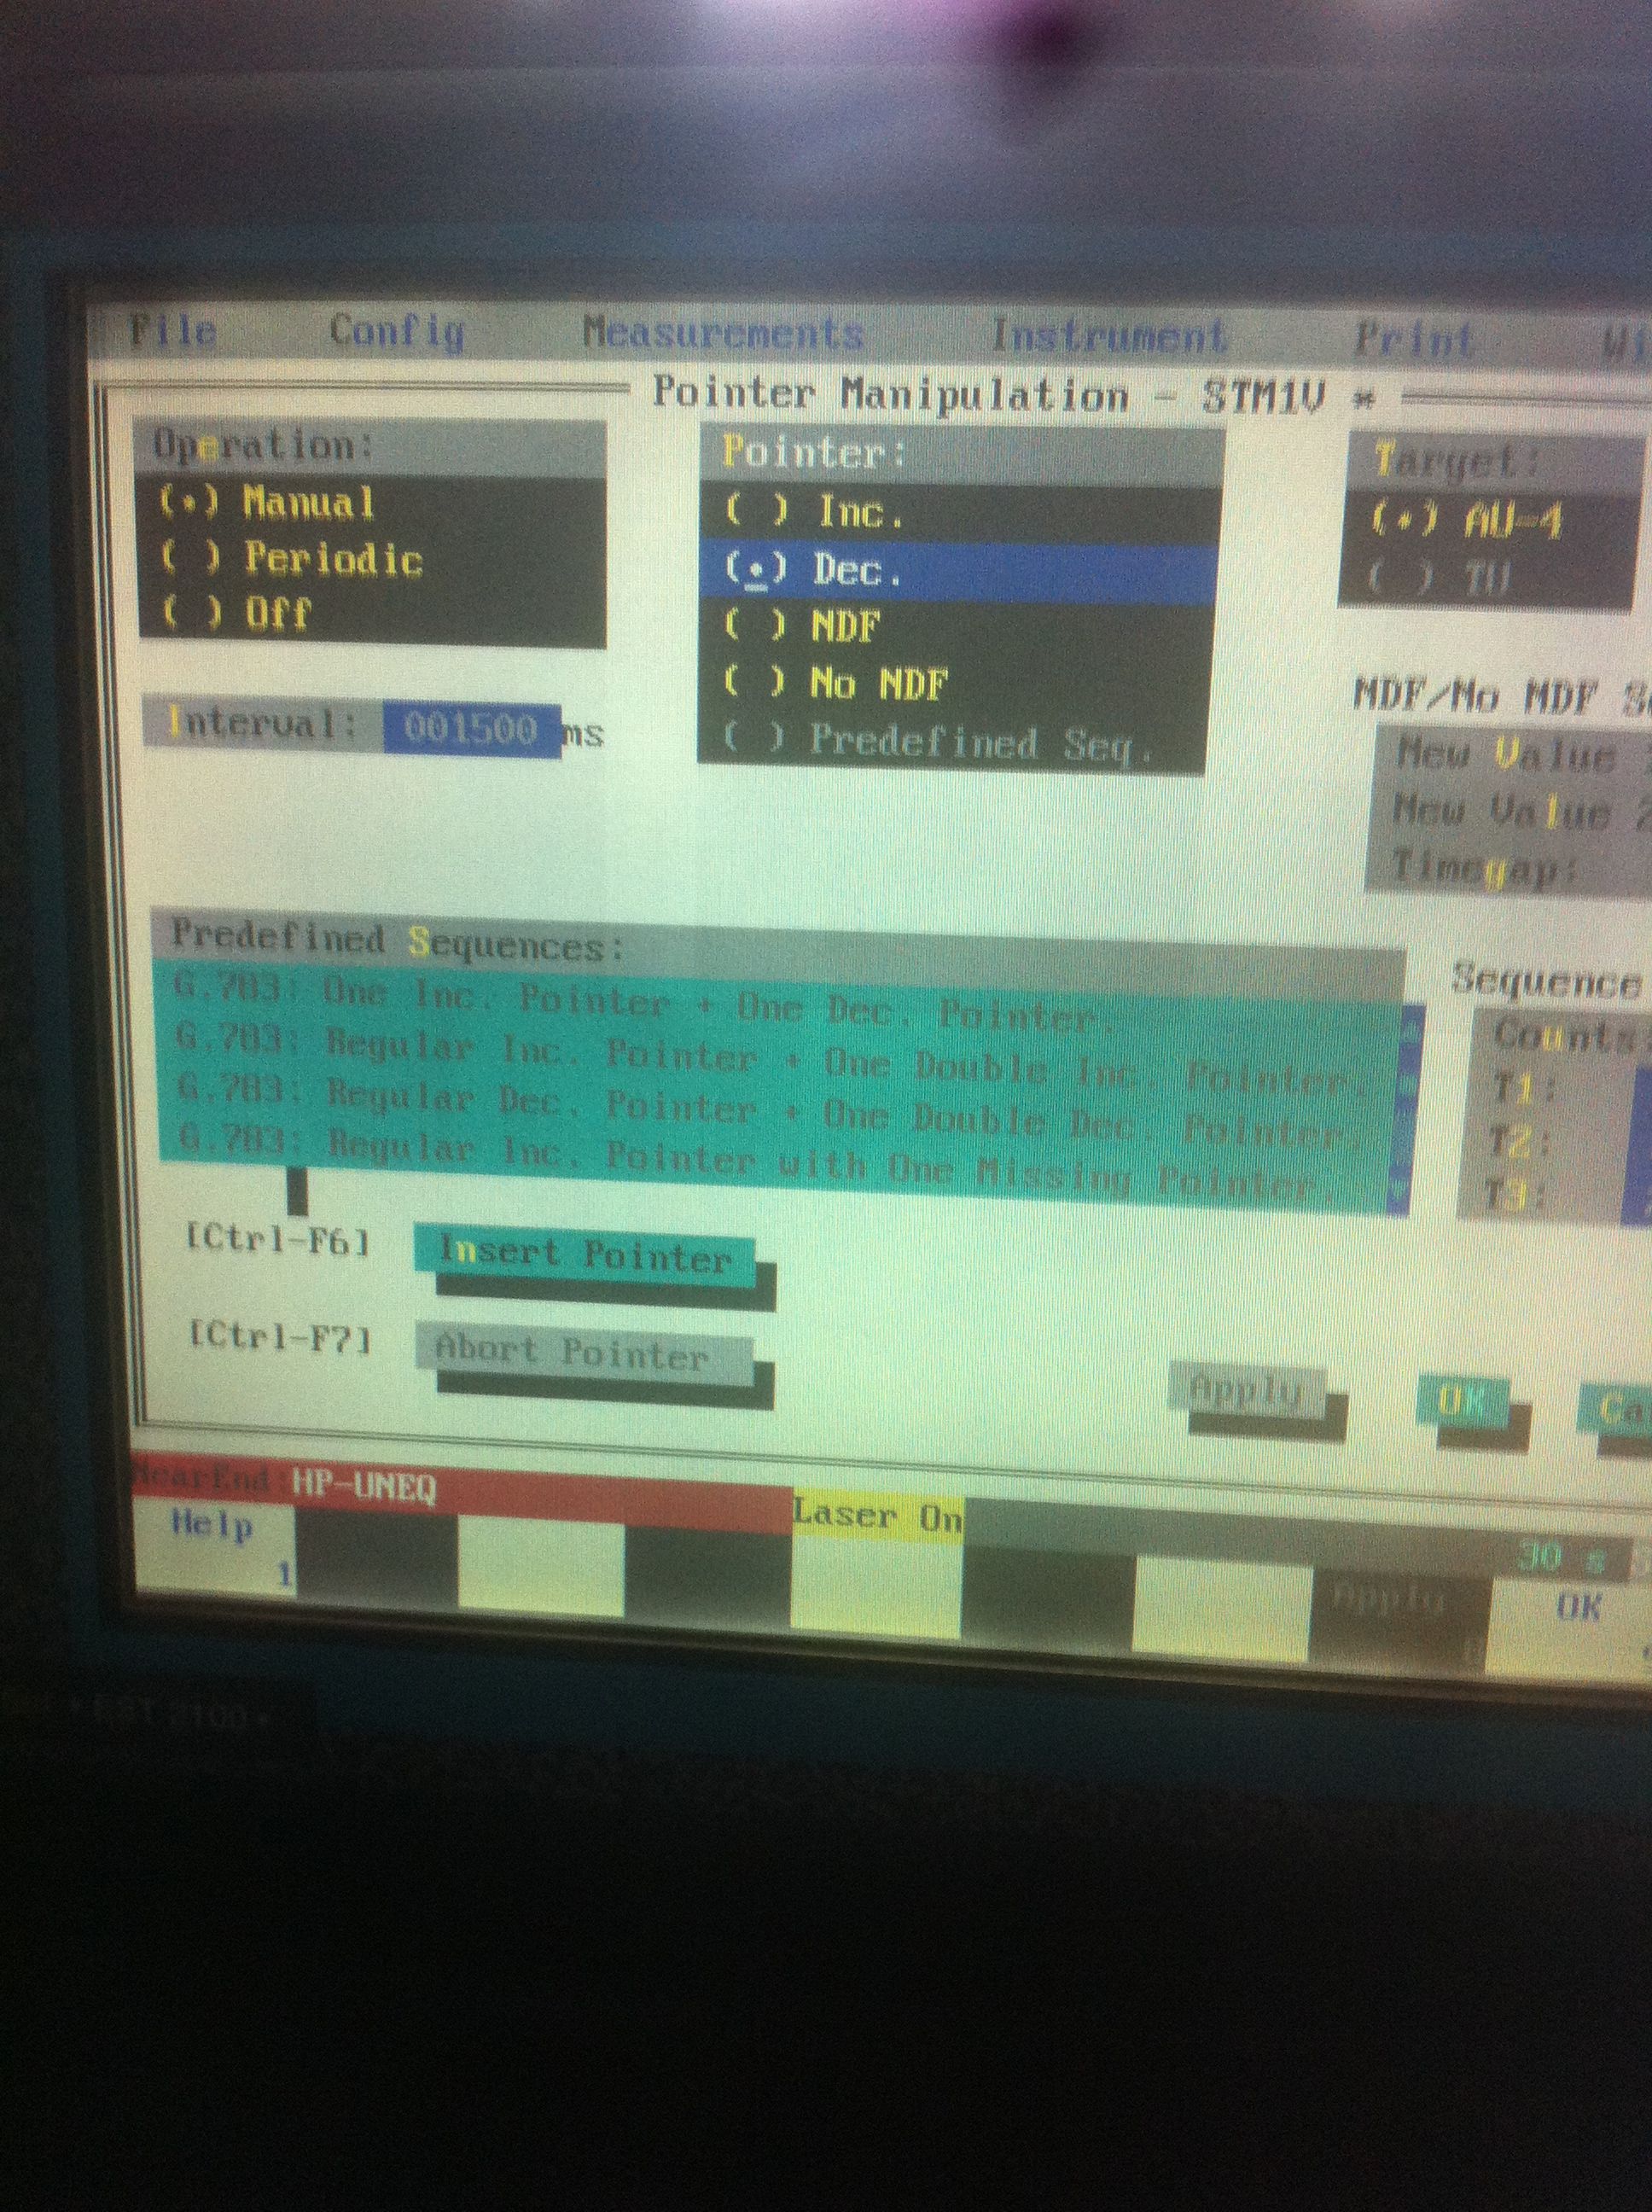
\includegraphics[scale=1]{sdh/IMG_1937.JPG} 

Zuerst Dekrementieren wir den Pointer was ein Pointer Justification Event auslöst und in TMNS im Performance Menu von AU-4 als -PJE-Erhöhung wahrzunehmen ist.
Entsprechend umgekehrt verhält sich das System für die Inkrementierung des Pointers. Im Versuch war zu erkennen das die ersten drei gesendeten Werte nicht in dem Perfomance-Fenster sichtbar waren. Dies ist darauf zurück zu führen das nur bei jedem vierten Rahmen eine Pointer-Aktivität durchgeführt wird. Also wurden die ersten drei als Ankündigung verstanden das nun der Pointer geändert wird. \todo{stimmt das denn auch?}

\subsubsection{Ändern des Taktes von Elmi}
Ändert man den Takt von Elmi auf den Internen so kann man einen hohen Sprung des +PJE Feldes beobachten. Dies zeigt das das System die beiden Multiplexer versucht zu synchronisieren. Dannach sieht man das das +PJE Feld weiter steigt, um etwa drei pro Sekunde. Die Erklärung dafür ist, das der interne Takt von Elmi etwas langsamer ist als der des anderen Multiplexern. So muss dieser positiv Inkrementieren um den Takt auszugleichen und das Netz synchron zu halten.

\subsubsection{kontinuierliches negatives Justieren bei Internem Takt}
Als letztes möchten wir gerne noch Versuchen was passiert wenn wir zusätzlich zu dem geändertem Takt noch negativ den Pointer justieren. Bei verwendung des internen Taktes von Elmi haben wir festgestellt das eine positive Pointerjustierung nötig ist um das Netz Synchron zu halten. Wenn wir nun aber auf der Sende Seite den langsameren Takt durch negativ Justierung ausgleichen kann man beobachten wie die benötigten Pointer-Aktivitäten sinken. Wenn man das Intervall entsprechend weit runter stellen würde könnte man den kompletten ausgleich zwischen den unterschiedlichen Takten erreichen. In dem Versuch haben wir beobachtet wie sich die Pointerjustierung auswirkt. Dies ist hier noch einmal Tabellarsich aufgeführt.

\begin{tabular}
Justierung & PointerAktivität \\
Inkrementierung & 5 Pointer pro Sekunde\\
Dekrementierung & 3 Pointer pro Sekunde \\
Ohne & 4 Pointer pro Sekunde \\
\end{tabular}

Die Tabelle zeigt auf das mit einer Positiven Justierung des Pointers zusätlich zu dem unteschiedlichen Takt eine noch höhere Pointer-Aktivität nötig ist um das System synchron zu halten. Wie oben beschreiben führt eine Dekrementierung zu einem annäherndem Ausgleich. Diese Aussage wird unterstützt wenn man sich die Spalte Ohne Justierung ansieht. Hier ist es etwa der Mittelwert der beiden anderen. 

\section{Fazit}
In den Versuchen wurde das bereits erlangte Wissen praktisch angewandt. Vor allem in dem Bereichen Pointer wurden die das Verständnis dafür sehr viel klarer und die Zusammenhänge eindeutiger. Allerdings waren die Versuche alle sehr klar definiert und die Erwartungen nicht überrascht.